\documentclass{article}

\usepackage{graphicx}
\usepackage{parskip}
\usepackage{amsmath}

\title{BSP Tree}
\author{Gerard Martin Teixidor}

\begin{document}
\maketitle

\section*{Overview}
A binary space partitioning (BSP) tree, is a data structure which subdivides space into convex subspaces by using hyperplanes~\cite{original}. This data structure can be seen as a generalization of a \textit{k}-d tree which, unlike a \textit{k}-d tree, the orientation and position of the spiting planes are arbitrary.

In a BSP tree, each inner node represents an hyperplane that splits the space into two half-spaces. The right child represents the positive half-space, while the left child represents negative half-space. The leaf nodes, unlike the inner nodes, nodes does contain any information about the hyperplane and represent a convex subspace.

\begin{figure}[h]
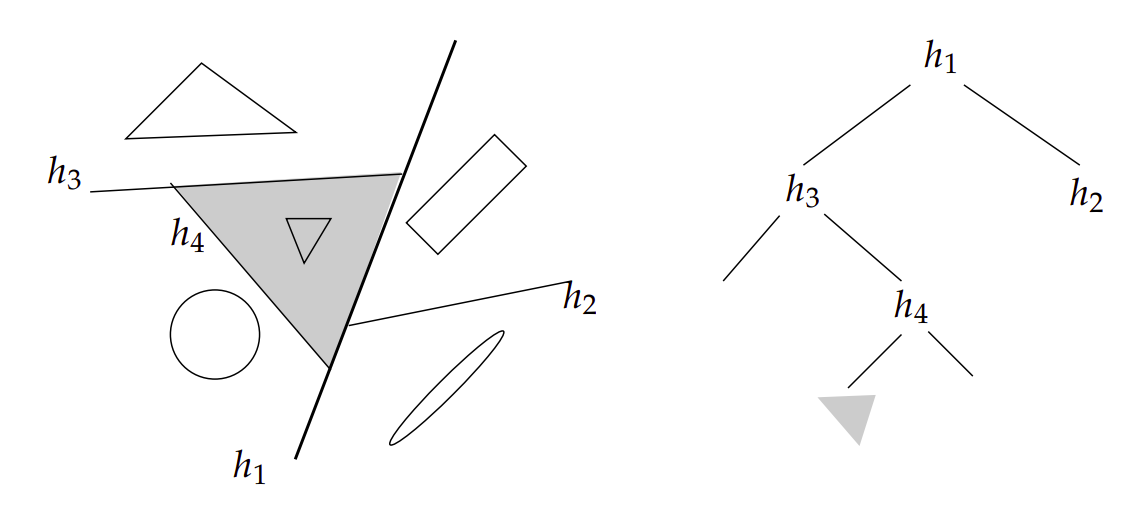
\includegraphics[width=0.9\linewidth]{bsp_tree.png}
\caption{Example of a BSP tree.}
\end{figure}

Because of the freedom of choosing the position and orientation of the hyperplanes, a common approach is to use the planes defined by the input data. Given a set of polygons as the input data, when all the hyperplanes are polygons from the input data, it is called an auto-partition BSP tree.

In the computer graphics field, BSP trees are used in multiple applications. The most common applications are:

\begin{description}
\item[Constructive solid geometry] Auto-partition BSP trees allow to represent volumetric polygonal closed objects by defining if a space space region is inside or outside the object. This representation also allows to check very efficiently if a point belongs inside or outside the object. Figure~\ref{object} shows an example of a 2D BSP tree representing an object.

\item[Boolean operations] Another interesting property of an object represented by a BSP tree is the ability to perform very efficiently boolean operation between objects. Given two objects, $A$ and $B$, being able to perform the boolean operations $\{\cup, \cap, \setminus, \ominus\}$. As a simple overview, the main idea behind this operations is to split one of the two BSP tree by the planes of the other BSP tree, and merging them with the corresponding boolean operation.

\item[Visibility priority] When rendering the polygons on the screen, an auto-partition BSP tree can be used to determine the drawing priority of those polygons~\cite{siggraph}.
\end{description}

\begin{figure}
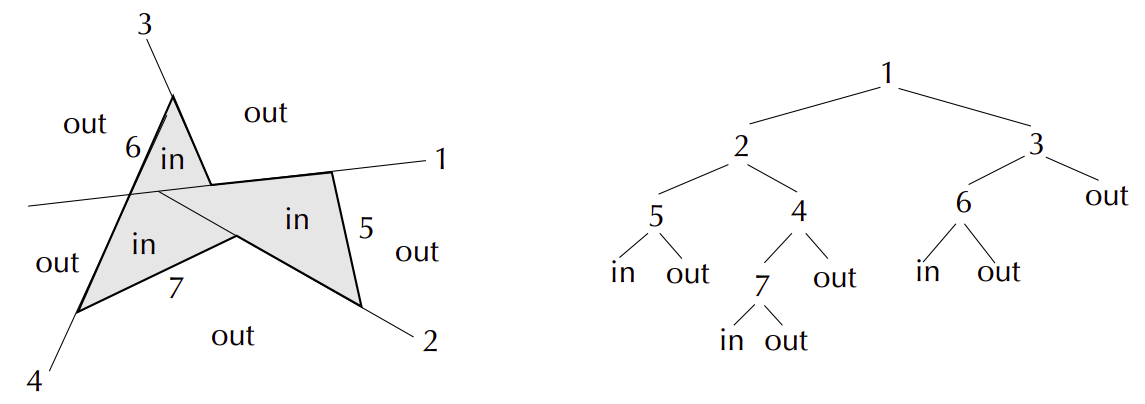
\includegraphics[width=\linewidth]{bsp_tree_object.png}
\caption{Auto-partition BSP tree which represents a closed object.}
\label{object}
\end{figure}

\subsection*{Visibility priority}
In computer graphics, the visibility problem of a 3D scene consists on defining which parts of the geometry are going to be visible on screen. The painter's algorithm allows to solve this problem by painting those polygons from back to front by overdrawing those portions of the screen which are occluded by the polygons painted on top. 

In static scenes, an auto-partition BSP tree can be used to solve this problem since it stores implicitly the polygon painting order from any view point.

\subsubsection*{Generation}
Given a set of polygons as the input data, to generate an auto-partition BSP the following algorithm is performed:
\begin{enumerate}
\item A polygon is chosen from the list.
\item For each other polygon in the list:
\begin{enumerate}
\item If the polygon is completely in front of the hyperplane, it is added to the right child.
\item If the polygon is completely behind the hyperplane, it is added to the left child
\item If the polygon intersects with the hyperplane, the polygon is split and each new fragment is added to the corresponding child.
\item If the polygon lies in the plane, is added tot the list of polygons of that node.
\end{enumerate}
\item This algorithm is applied recursively to each child until there is only one polygon on each node.
\end{enumerate}

It is important to note that the selection of the polygon which specifies the hyperplane (step~1) is going to impact the number of fragments generated down the tree. There exist different heuristics which try to minimize the number of splits.

\subsubsection*{Image generation}
Once the BSP tree has been generated, the tree can be traversed in linear time in order to determine the visibility priorities of each polygon.

From the root node:
\begin{enumerate}
\item If the view location is in front of the hyperplane
\begin{itemize}
\item Paint the left child (behind) polygons recursively.
\item Paint the current node polygons. 
\item Paint the right child (int front) polygons recursively.
\end{itemize}
\item If the view location is behind the the hyperplane
\begin{itemize}
\item Paint the right child (int front) polygons recursively.
\item Paint the current node polygons. 
\item Paint the left child (behind) polygons recursively.
\end{itemize}
\end{enumerate}

To check if the view is in front or behind the plane, is just a matter com computing the singed distance of a point with respect of the hyperplane.

\section*{Personal opinion}
Nowadays the BSP trees are not that relevant in the computer graphics field and seams to be taken over by other more advanced data structures. This is obvious in the case of the visibility problem. Nowadays the default solution to this problem is the use of the Z-Buffer. This alternative is not a data structure by itself, but instead is a hardware accelerated GPU buffer. This GPU buffer allows to perform the priority sorting directly on the GPU, and at pixel level, with a minimum performance penalty.

Also, in the case of solid modeling, the rendering of those objects does not require them to be represented by BSP trees. Like with the visibility problem, this rendering can be perform with  object primitives and the help of another hardware buffer called stencil buffer.

\section*{Experiments}
One of the main problem with BSP trees is the size of the tree. In the case of a BSP tree constructed from a set of polygons, this size of the tree can be much larger than the number of polygons $n$ due to the hyperplanes splitting those polygons. While the number of fragments in an 2D auto-partition BSP tree is bounded $O(n^2 \log n)$, in higher dimensions the known bound is much wider. In the case of 3D BSP trees they can be as many as $O(n^2)$ fragments.

Even thought there can be as many as a quadratic number of fragments, the reality is that, due to the principle of locality, BSP trees contain much fever fragments. The principle of locality states that polygons are smaller compared to the whole space.

The implemented experiment tries to show this reality by constructing multiple BSP trees and comparing the number of polygons with respect to the number of fragments. The BSP trees generated are auto-partitions BSP trees from real models and from a set of random polygons.

As we can see in the results (Table~\ref{results}) we can see that in reality, the number of fragments is far from the upper bound. Also this experiment shows the principle of locality as we can see that, when using random polygons, the number of fragments increase with respect to the models. This is due to the models being composed by small polygons, while the size of the random polygons is variable.

\begin{table}
\centering
\begin{tabular}{|c|c|}
\hline
\textbf{Polygons} & $\boldsymbol{Fragments/Polygons^2}$ \\
\hline\hline
Monkey & 0.004\% \\
Sphere & 0.028\% \\
Teapod & 0.017\% \\
Random & 1.633\% \\
\hline
\end{tabular}
\caption{Table showing the number of fragments generated by the BSP tree.}
\label{results}
\end{table}

\section*{Conclusions}
Even being forgotten nowadays, BSP trees are an interesting very data structure which still are being used. It seams that one of the causes of its decrease in popularity is that many applications now uses more advanced an efficient techniques which allow to parallelize the computation (e.g. Z-Buffer for the visibility problem).

\bibliographystyle{unsrt}
\bibliography{report.bib}

\end{document}